
本章では,SAS-L2での認証方法について説明する.
\section{SAS-L2(SimpleAnd Secure password authentication protocol,Light processing version, type 2)の概要}
SAS-L2とは,高知工科大学の清水明宏教授が提案した処理負荷が特に小さいワンタイムパスワード認証方式SAS-Lの一つである\cite{sas-l}.
表\ref{tb:sashikaku}から分かるように,従来のSASと比較し,特に被認証者側の処理負荷が小さい認証方式である.

\begin{table}[H]
\centering
\caption{SAS-2とSAS-L2の演算回数の比較}
\label{tb:sashikaku}
\begin{tabular}{|c|c|c|c|c|c|c|} \hline
 & \multicolumn{3}{c|}{ユーザー} & \multicolumn{3}{c|}{サーバー} \\
 \cline{2-7}
  & ハッシュ関数 & XOR & 加算 & ハッシュ関数 & XOR & 加算\\ \hline
  SAS-2 & 2 & 3 & 0 & 1 & 2 & 0\\ \hline
  SAS-L2 & 0 & 2 & 2 & 1 & 3 & 2\\ \hline
  \end{tabular}
  \end{table}

処理性能の低いIoT機器において,極めて小さい処理負荷で暗号鍵の配送が実現できる.
バーナム暗号などと組み合わせて暗号系を組むことで,処理能力の低いIoT機器へ暗号化通信機能を付加できる\cite{sas-l}.
SAS-L2は,認証者と被認証者にあらかじめ初回認証情報と初回秘匿情報の登録を行う初期登録処理と,
以降の認証処理から構成される.
認証者と被認証者は,以降でそれぞれサーバー,ユーザーと定義する.


\subsection{初期登録処理}
SAS-L2の初期登録処理のフローチャートを図\ref{fig:sas-l2_syoki}に示す.

\begin{figure}[H]
\begin{center}
	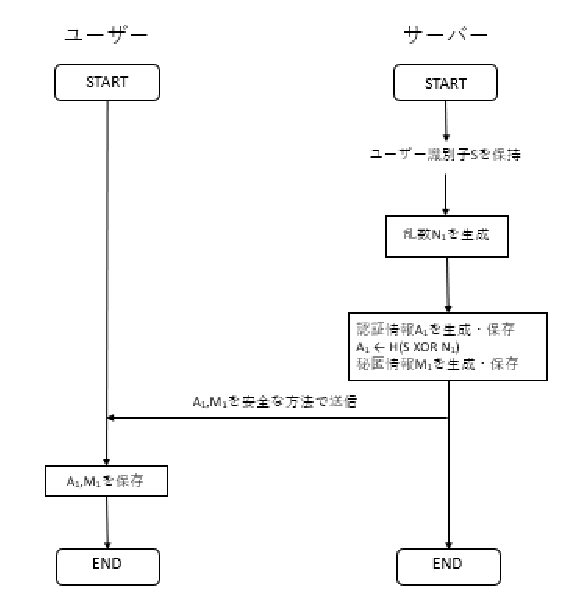
\includegraphics[height=100mm]{sas_l2_syoki.eps}
	\caption{初期登録処理の手順}
\label{fig:sas-l2_syoki}
\end{center}
\end{figure}

初期登録は,以下の手順に沿って処理が行われる.
\begin{enumerate}
	\item サーバーはユーザー識別子$S$を保持する.
	\item サーバーは初期認証用の乱数$N_1$を生成する.
	\item サーバーは,ユーザー識別子$S$と乱数$N_1$の排他的論理和にハッシュ関数を適用し,
	初期認証用の認証情報$A_1$を生成・保存する.
	\item サーバーは初期認証用の秘匿情報$M_1$を生成・保存する.
	\item サーバーは認証情報$A_1$と秘匿情報$M_1$を安全な方法でユーザーに送信する.
	\item ユーザーはサーバーから受信した認証情報$A_1$と秘匿情報$M_1$を保存する.
\end{enumerate}
初期登録の終了後,以降は認証処理が行われる.

\subsection {認証処理}
SAS-L2の$n$回認証時のフローチャートを図\ref{fig:sas-l2_ninsyo}に示す.
$N_n$,$A_n$,$M_n$はそれぞれ$n$回目認証用の乱数,認証情報,秘匿情報である.

\begin{figure}[H]
\begin{center}
	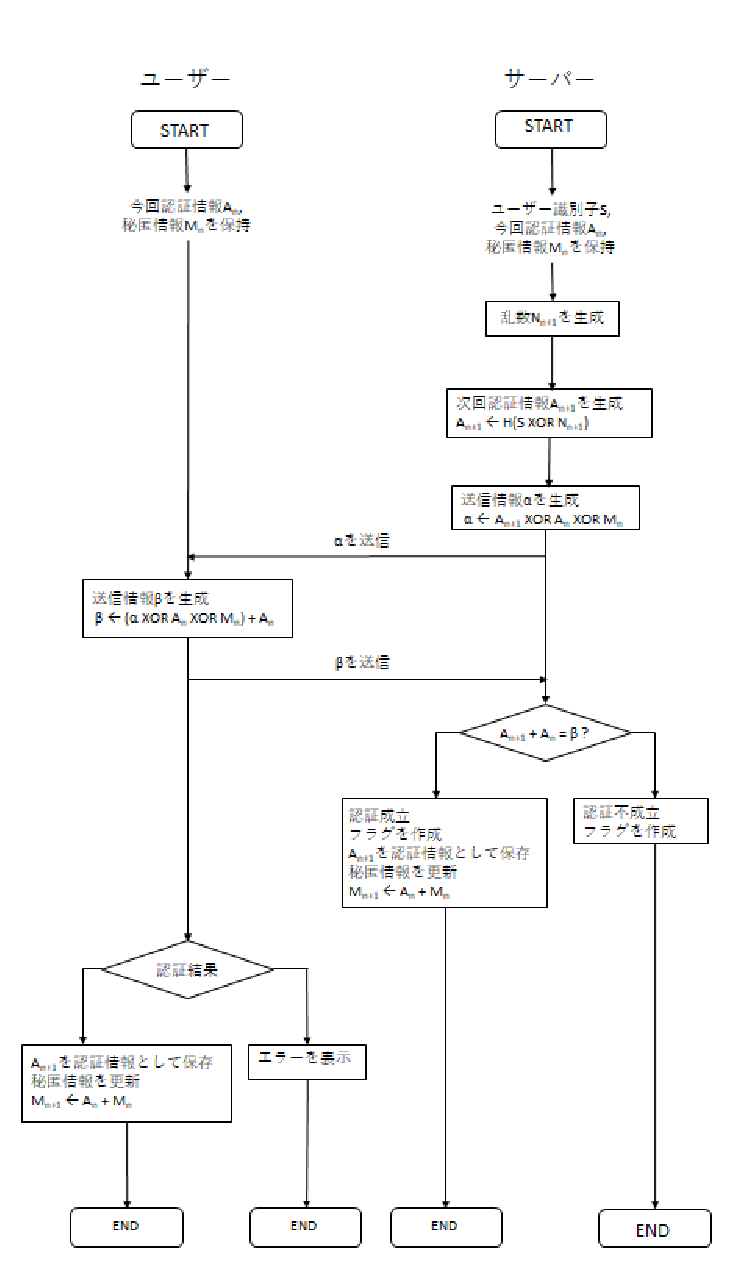
\includegraphics[height=200mm]{sas_l2.eps}
	\caption{認証手順}
\label{fig:sas-l2_ninsyo}
\end{center}
\end{figure}

認証は,以下の手順に沿って処理が行われる.
\begin{enumerate}
	\item サーバーはユーザー識別子$S$と認証情報$A_n$と秘匿情報$M_n$を保持している.
	ユーザーは認証情報$A_n$と秘匿情報$M_n$を保持している.
	\item サーバーは次回認証用の乱数$N_{n+1}$を生成する.
	\item サーバーは,ユーザー識別子$S$と乱数$N_{n+1}$の排他的論理和にハッシュ関数を適用し,
	次回認証用の認証情報$A_{n+1}$を生成する.
	\item サーバーは認証情報$A_{n+1}$,$A_n$と秘匿情報$M_n$の排他的論理和を演算し,$\alpha$を生成する.
	\item サーバーは$\alpha$をユーザーに送信する.
	\item ユーザーはサーバーから受信した$\alpha$と認証情報$A_n$,秘匿情報$M_n$の排他的論理和($\alpha \oplus A_n \oplus M_n(=A_{n+1})$)
	と認証情報$A_n$の算術加算により,$\beta$を生成する.
	\item ユーザーは$\beta$をサーバーに送信する.
	\item サーバーはユーザーから受信した認証情報$A_{n+1}$と保持していた$A_n$の加算を$\beta$と比較し,
	一致すれば認証成功し以下の処理が実行される.不一致ならば認証は不成立となり,
	以下の処理は実行されない.
	\item ユーザーは$\alpha$と認証情報$A_n$,秘匿情報$M_n$の排他的論理和を演算し次回認証用の認証情報$A_{n+1}$を生成し保存する.
	認証情報$A_n$と秘匿情報$M_n$の加算を行い,次回認証用の秘匿情報$M_{n+1}$を$M_n$の代わりに保存する.
\end{enumerate}
以上の処理で1回の認証が終了し,次回以降も認証を行う度に以上の処理を繰り返す.
